\documentclass[smallextended]{svjour3}       % onecolumn (second format)
%\documentclass[twocolumn]{svjour3}          % twocolumn
%
\smartqed  % flush right qed marks, e.g. at end of proof...test
%
\usepackage{graphicx}
\usepackage{makecell}
\usepackage{hyperref}
\usepackage{todonotes}
%
% \usepackage{mathptmx}      % use Times fonts if available on your TeX system
%
% insert here the call for the packages your document requires
%\usepackage{latexsym}
% etc.
%
% please place your own definitions here and don't use \def but
% \newcommand{}{}
%
% Insert the name of "your journal" with
% \journalname{myjournal}
%
\begin{document}

\title{Discovering language resources using Linghub}
\titlerunning{Linghub}

\author{John P. McCrae       \and
    Markus Ackermann         \and
    Philipp Cimiano          \and
    Martin Br\"ummer         \and
    Victor Rodr\'iguez Doncel\and
    Daniel Vila              \and
    Gabriela Vulcu           \and
    Andrejs Abele            \and
    Paul Buitelaar           \and
    Luca Matteis             \and
    Tiziano Flati            \and
    Jorge Gracia}


    \authorrunning{McCrae et al.}

\institute{John P. McCrae, Gabriela Vulcu, Andrejs Abele, Paul Buitelaar \at
              Insight Centre for Data Analytics \\
              National University of Ireland Galway \\
              \email{john@mccr.ae, \{gabriela.vulcu,
              andrejs.abele\}@insight-center.org}
           \and
           Markus Ackermann \at
              Institute for Applied Informatics \\
              Leipzig University \\
              \email{ackermann@informatik.uni-leipzig.de}
            \and
            V\'ictor Rodr\'iguez Doncel, Jorge Gracia \at 
                Ontology Engineering Group \\
                Polytechnic University of Madrid \\
                \email{\{vrodriguez, jgracia\}@fi.upm.es}
            \and
            Luca Matteis, Tiziano Flati \at
                University of Rome ``La Sapienza'' \\
                \email{\{matteis, flati\}@di.uniroma1.it}
            \and\\
            John P. McCrae, Philipp Cimiano \at
                Cognitive Interaction Technology, Excellence Cluster \\
                Bielefeld University \\
                \email{cimiano@cit-ec.uni-bielefeld.de}
}

\date{Received: date / Accepted: date}
% The correct dates will be entered by the editor


\maketitle

\begin{abstract}
\keywords{First keyword \and Second keyword \and More}
\end{abstract}

\section{Introduction}

The study of language and the development of natural language processing (NLP)
applications requires access to language resources (LRs). Recently, several
digital repositories that index metadata for LRs have emerged, supporting the
discovery and reuse of LRs. One of the most notable of such initiatives is
META-SHARE~\cite{federmann2012meta}, an open, integrated, secure and interoperable exchange
infrastructure where LRs are documented, uploaded, stored, catalogued,
announced, downloaded, exchanged and discussed, aiming to support reuse of
LRs\footnote{\url{http://www.meta-share.eu}}. Towards this end, META-SHARE has developed a rich
metadata schema that allows aspects of LRs accounting for their whole lifecycle
from their production to their usage to be described. The schema has been
implemented as an XML Schema Definition (XSD) and descriptions of specific LRs
are available as XML documents. Yet, META-SHARE is not the only source for
discovering LRs and their descriptions; other sources include the catalogs of
agencies dedicated to LRs promotion and distribution, such as
ELRA\footnote{\url{http://www.elra.info}} and
LDC\footnote{\url{https://www.ldc.upenn.edu/}}
other infrastructures such as the CLARIN Virtual Language Observatory
(VLO)~\cite{van2012semantic}, the Language Grid~\cite{ishida2006language} and
Alveo\footnote{\url{http://alveo.edu.au/}}, the Open Language Archives
Community~\cite[OLAC]{simons2003open}, catalogs with crowd-sourced metadata,
such as the LRE-Map~\cite{calzolari2012lre}, and,
more recently, repositories coming from various communities (e.g.
OpenAire~\cite{manghi2010infrastructure},
EUDAT\footnote{\url{http://www.eudat.eu}} etc.). The metadata schemes of all these sources vary with respect to
their coverage and the set of specific metadata captured. Currently, it is not
possible to query all these sources in an integrated and uniform fashion. The
Web of Data is a natural scenario for exposing LRs metadata in order to allow
their automated discovery, share and reuse by humans or software agents and the
benefits of this model including interoperability.

In this paper, we are concerned with how to facilitate the discovery of language
resources for a particular task. Given the fact that metadata records for
resources are distributed among different catalogs and repositories makes the
task of finding a particular resource meeting certain requirements very
challenging. This is shown by the fact that many emails to dedicated
mailing lists such as the copora mailing list contain requests for resources
meeting certain desiderata with respect to type of resource (corpus, dictionary,
parallel text, etc.), language, size (in tokens or sentences), etc.
So far, no repository that allows discovery of resources across repositories has
been available. We have closed this gap by developing Linghub, a linked data
based portal that indexes and aggregates metadata entries from different
repositories including META-SHARE, the CLARIN VLO, LRE-Map and Datahub.io.

Parts of the Linghub as a technical system has been described
before~\cite{mccrae2015reconciling,mccrae2015linghub}. Linghub not
only indexes the metadata entries, but also harmonizes the information by
mapping it to standard semantic web vocabularies as well as to an ontology to
describe language resources that has been developed on the basis of the existing
Metashare schema~\cite{mccrae2015ontology}.
For this, it relies on state-of-the-art word sense disambiguation methods to
support the normalization of data. 

One of the crucial technologies that enables this integration is that of
RDF~\cite{klyne2006resource} and linked data. Linked data is based on four fundamental princi-
pals~\cite{bizer2009linked}.

\begin{enumerate}
    \item Use Uniform Resource Identifiers  to identify everything in a resource, thus
        ensuring that every element of the resource can be identified in a standard
        manner.
    \item Furthermore, use HTTP URLs as they require the association with domain names,
        ensuring that the data can be clearly traced to its host and thus someone
        responsible for that dataset.
    \item Ensure that URLs resolve, in the sense that when typed in to a web browser an
        appropriate description of the resource is obtained. Ideally the server should
        detect (using content negotiation) the type of the user and provide HTML
        results for humans and XML or JSON for software agents.
    \item Provide links to other resources so that it is possible to identify
        commonalities between resources and to handle issues of semantic
        interoperability and provenance.
\end{enumerate}

Linked data makes a highly appropriate model for the task of integrating information
about language resources as it is natural that this would be handled by means
of a web portal and thus stable URLs for resources are easily decided. It is
obvious that HTML descriptions should be provided and in order to meet
use cases for automatic training of NLP systems, we find the provision of a
machine-readable API also of vital importance. Finally, links to other resources
are vital to not only provide links back to the source records, but also to ensure
that users can find resources for their needs.

In this paper, besides describing Linghub and the semantic normalization
methods used, we provide an evaluation of the
ability of Linghub to answer the needs of actual users seeking language
resources meeting certain criteria. For this, we have analyzed user requests
for resources issued on Corpora List and analyzed in how far Linghub is
able to answer them. This evaluation is the main contribution of the current
paper. We are not aware of any similar evaluation conducted in the context of
repositories of language resources, so that to our knowledge this is the first
attempt to evaluate the ability of a repository to answer requests for language
resources.

%Most natural language processing systems rely to some extent on the use of
%datasets in the form of language resources to train themselves for a specific
%language or domain and as such the challenge of adapting a tool requires the
%discovery of suitable langauge resources. Unfortunately, language resources are
%often published independently by researchers and are thus difficult to discover
%with standard information retrieval mechansims (e.g., search engines) and can
%quickly become unavailable after a short period of time. There have been a couple of approaches to
%record information about language resources and they can be broadly divided into two approaches, which we
%term the \emph{curatorial} approach and the \emph{crowd-sourcing} approach. The
%curatorial approach relies on the use of expert ``curators'' to document the
%existing resources and create high quality \emph{metadata} about the resources
%that are available given time and funding for these efforts. This approach has the advantage that it produces
%comprehensive descriptions of the resources but has a crucial drawback that it
%is difficult for curators to describe, or even know about, all resources that
%are available. In contrast, the crowd-sourcing approaches relies on users to
%document resources in central catalogues ensuring that there are indexes where
%users can easily access these resources. This can provide significantly more
%coverage of the language resources that are available but has an issue with
%quality of the documentation of the resources is often weak, as the metadata
%descriptions are not created by experts but by users in an `ad-hoc' manner.
%
%As both approaches have some clear and significant disadvantages it seems
%natural to ask if we can combine the advantages of these approaches.
%Thus, we propose an \emph{integral} approach that relies on
%collecting metadata about language resources from multiple sources and
%integrating them into single records. This relies on the use of state-of-the-art
%techniques including word sense disambiguation in order to link the resources
%and ensure that they refer to values in the same way. For example, a resource
%may have a property called `language' but its value may be a language name in
%English or another language or an identifier such as an ISO 639
%code~\cite{gordon2005ethnologue} of which there are 3 variants. 
%
%One of the crucial technologies that enables this integration is that of
%RDF~\cite{klyne2006resource} and linked data. Linked data is based on four fundamental
%principals~\cite{bizer2009linked}.
%
%\begin{enumerate}
%    \item Use Uniform Resource Identifiers to identify everything in a resource,
%        thus ensuring that every element of the resource can be identified in a
%        standard manner.
%    \item Furthermore, use HTTP URLs as they require the association with domain
%        names, ensuring that the data can
%        be clearly traced to its host and thus someone responsible for that
%        dataset.
%    \item Ensure that URLs resolve, in the sense that when typed in to a web
%        browser an appropriate description of the resource is obtained. Ideally
%        the server should detect (using content negotiation) the type of the
%        user and provide HTML results for humans and XML or JSON for software
%        agents.
%    \item Provide links to other resources so that it is possible to identify
%        commonalities between resources and to handle issues of semantic
%        interoperability and provenance.
%\end{enumerate}
%
%Linked data makes a very good fit for the task of integrating information about
%language resources as it is natural that this would be handled by means of a web
%portal and thus stable URLs for resources are easily decided. It is obvious that
%HTML descriptions should be provided and in order to meet use cases for
%automatic training of NLP systems, we find the provision of a machine-ready API
%also of vital importance. Finally, links to other resources are vital to not
%only provide links back to the source records, but also to ensure that users can
%find out more information about the properties used to describe language resources.
%
%In this paper, we present the Linghub system, which aims to integrate language
%resources by means of linked data and thus provide a single accessible portal
%for both humans and machines to find suitable language resources or their needs.

This paper is structured as follows: Firstly, in Section~\ref{related-work} we
will discuss some of the existing related work in particular focussing on the
metadata repositories that we will integrate and in
Section~\ref{data-collection} we will describe how we collected the data. In
Section~\ref{modelling} we derive a single data model based on existing
standards that will allow us to combine all the resources and then in
Section~\ref{harmonization} we will show our procedure for harmonizing these
resources. We will describe the web portal in
Section~\ref{linked-data-interface}. In Section~\ref{evaluation}, we provide a
thorough evaluation of the system based on real-world queries and thus show the
effectiveness of our approach, and finally we conclude in
Section~\ref{conclusion}.\footnote{Some results in this paper have been
    previously published in the following workshop papers
    \cite{mccrae2015linghub,mccrae2015reconciling,mccrae2015ontology}. The results
    and methods are expanded and combined in this paper in line with the journal
    guidelines. In addition, Section~\ref{evaluation} provides a novel
evaluation of the system.}

\section{Related Work}
\label{related-work}

Harmonization has been a topic of significant importance in managing metadata
and it has been noted in several domains that the task of combining metadata
from multiple sources. Nilsson~\cite{nilsson2010interoperability} proposed
a framework for this, where he argues that syntax is of little importance and
that harmonization primarily needs to be conducted on a semantic level and he
concludes that RDF forms a good model to achieve this. Khoo and
Hall~\cite{khoo2010merging} worked on merging the Internet Public Library and
the Librarian’s Internet Index and conclude that such resource is very
`ad-hoc' and `resource intensive'. Nogueras et
al.~\cite{nogueras2004metadata} similarly developed `crosswalks' for
geographic data and stress the need for formal modelling such as ontologies for
verifying such crosswalks. Chan and Zeng~\cite{chan2006metadata} also focus
on the use of crosswalks and its use in provding optimal access to data. 

One of the key issues in this has between `monolithic' metadata schemas where
one organization has developed and maintained a single and fixed schema for
representing metadata. Such standards, frequently defined by fixed XML DTDs and can
be useful in providing a minimal level of description between multiple resources
however they cannot by their very nature capture all the complexities of the
representation of metadata. A highly successful instance of this is Dublin
Core~\cite{weibel1998dublin}, where a small fixed set of properties has found
use in a wide variety of applications.
Instead, some experts have recommended open schemas\cite{brooks2006towards}:

\begin{quote}
``A larger set of ontologies sufficient for particular purposes should
be used instead of a single highly constrained taxonomy of values.''
\end{quote}

On the other hand open schemas are difficult
as they can often lead to a large number of identifiers for the same properties
or concepts, which has lead to the failure of such schemes in the
past~\cite{kemps2008isocat}. The proposal of linked data to allow for additional
properties to be dereferenced and thus for extra information about their
semantics to be extracted has formed the basis of the Semantic Web. In this
context, there have been several vocabularies defined for representing metadata
about data resources, notably the VoID model~\cite{alexander2011describing}, the
DCAT model~\cite{maali2014data} and its recent extension
DataID~\cite{brummer2014dataid}. These have the possibility to enable more
flexible description of language resources and it has even been suggested that
these resources could be automatically collected~\cite{jenkins1999automatic}.

In the context of language resources, there have been a number of attempts to
collect generic metadata about language resource. Firstly
META-SHARE~\cite{gavrilidou2012meta,piperidis2012meta}, which has relied on
creating descriptions of language resources manually but has still be able to
describe in detail a large number of language resources. Another approach that
relies on institutional collection of metadata was taken by the CLARIN project,
whose \emph{Virtual Language Observatory}~\cite{van2012semantic} collects
metadata from a number of host institutes by means of
OAI-PMH~\cite{sompel2004resource} with a small amount of harmonization provided
by the \emph{CMDI Component 
Specification Language}~\cite{broeder2012cmdi}. A similar project called
SHACHI~\cite{tohyama2008shachi} has worked on collecting resources on Asian
languges. Another approach in this area is the use of International Standardized
Language Resource Numbers~\cite[ISLRN]{choukri2012using}, where basic metadata
has been collected about each resource and they have all been assigned a single
number.

As an alternative to the institutional approach, some resources have relied on
self-reporting of resource metadata, most notably the
LRE-Map~\cite{calzolari2012lre}, which collects information from authors at
major research conferences in computational linguistics and as such they are
able to collect information on a wide variety of language resources but often
leads to quality issues. A similar project, the Open Language Archive
Community~\cite[OLAC]{piperidis2012meta} is inbetween both approaches collecting
resources from a wide community but trying to bring them into a very fixed
schema for their resources. Finally, we note the work of the \emph{Open
Linguistics Working Group}~\cite{chiarcos2012open} a community, which has
promoted the use of open data and produced a `cloud diagram' showing the
adoption of linked data language resources over the last four years.

\section{Data Collection}
\label{data-collection}

In order to realize the goal of providing comprehensive metadata about language
resources, it is necessary to collect metadata from a wide range of sources. In
parrticular, we chose four main sources, primarily because these resources have
been released under an open license. These resources are:

\begin{description}
    \item[META-SHARE] A resource created by the META-NET project,  the resource
        provides deep and detailed descriptions of language resources that have
        primarily been constructed by hand.
    \item[CLARIN VLO] The Virtual Language Observatory by the CLARIN project is
        a collection of resources drawn from a wide variety of insitutes
        participating in the CLARIN project. In general, the data has been
        manually curated by the individual contributors and only limited
        integration has been made between the resources. As such the records are
        very different in detail and size.
    \item[Datahub.io] This site is an instance of CKAN used primarily to track
        open and linked data. Most of the data is not of relevance to language
        resources and as such we apply filters to extact the relevant datasets.
    \item[LRE-Map] The LRE-Map was collected by participants at several NLP
        conferences in the last few years. Unfortunately, only the data from
        LREC-2014 is available under an open license and the method of collection has
        lead to significant issues with data quality.
\end{description}

In addition, we have a number of other sources that we investigated for the
experiments described in this paper but unfortunately cannot release through the
Linghub portal due to licensing.

\begin{description}
    \item[LRE-Map] Several other conferences of data are accessible on the Web
        and we have scraped the relevant data.
    \item[OLAC] The Open Language Archives Community collects a large amount of
        data, but clearly states that its own data is not ``open''. Fortunately
        most of the data is also available from CLARIN and other sources.
    \item[ELRA/LDA] We also experimented partially with the catalogue of
        resources provided by theses commercial data providers.
\end{description}

In the following section we describe the format of the resources and the
difficulty in consolidating them with our model.

\begin{table}
\resizebox{0.94\textwidth}{!}{\begin{minipage}{\textwidth}
    \begin{tabular}{l|r|r|r}
        \thead{Source} & \thead{Records} & \thead{Triples} & \thead{Triples per \\ Record} \\
        \hline                                              
        META-SHARE &   2,442 &   464,572 & 190.2 \\
        CLARIN     & 144,570 & 3,381,736 &  23.4 \\
        Datahub.io &     218 &    10,739 &  49.3 \\
        LRE-Map    &   5,712 &    79,576 &  13.9 \\
    \end{tabular}
\end{minipage}}
    \caption{\label{tab:resource-sizes}The sizes of the resources in terms of
    number of metadata records and total data size}
\end{table}

\subsection{META-SHARE}

META-SHARE is provided primarily in a format described in
\cite{gavrilidou2012meta}, which is
and XML format and contains over 150 elements and as such is a highly complex XML
format. We developed a custom invertible framework called LIXR (pronounced
`elixir')~\footnote{http://github.com/liderproject/lixr}, which allows us to easily and
quickly define the conversion between META-SHARE and RDF. As a great many of the
elements defined in the META-SHARE schema are very unique many of the elements
have to be created in a new ontology, which we developed as the META-SHARE
ontology, which is described in \cite{mccrae2015ontology}. 

\subsection{CLARIN}

\begin{table}
\begin{tabular}{l|lc}
Component Root Tag & Institutes & Frequency \\
\hline
Song & 1 (MI) & 155,403 \\
Session & 1 (MPI) & 128,673 \\
OLAC-DcmiTerms & 39 & 95,370 \\
MODS & 1 (Utrecht)& 64,632 \\
DcmiTerms & 2 (BeG,HI) & 46,160 \\
SongScan & 1 (MI) & 28,448 \\
media-session-profile & 1 (Munich) & 22,405 \\
SourceScan & 1 (MI) & 21,256 \\
Source & 1 (MI) & 16,519 \\
teiHeader & 2 (BBAW, Copenhagen) & 15,998 \\
\end{tabular}
\

    \caption{\label{tab:clarin-resources}The relative number of resources in
    each of the schemas used by CLARIN}
\end{table}

CLARIN is also an XML format and is based on the CMDI metadata infrastructure as
defined by \cite{broeder2012cmdi}. This consists of a small shared amount of information and
a specific schema, which is normally unique to the data provider, with the
exception of Dublin Core metadata which is in two common schemas. The total size
and applicability of each of the schemas is given in Table
\ref{tab:clarin-resources} and we have developed export scripts for all of the
top 10 formats.

\subsection{LRE-Map}

The LRE-Map is described in \cite{calzolari2012lre} and is available partly as RDF, in
particular the data from LREC-2014 is available. Unfortunately, the integration
was not trivial as there were errors in the RDF~\cite{del2014lre}, in particular the use of
non-resolving URI schemes that had to be corrected. The older data is also
available on the web site and we obtained it by scraping the web site but were
advised that this data is not available under any open license.

\subsection{Datahub.io}

Datahub.io is an instantiation of the CKAN
software\footnote{\url{http://ckan.org}} and as such can
easily be accessed through the API and the RDF version of each metadata using
the DCAT vocabulary can be accessed. As such the import of this data is quick
and can be done at regular intervals.

\subsection{Others}

In addition, we looked at three other sources that cannot be included in the
public release of Linghub due to the licensing issues. These are OLAC, which
uses an XML format and much like CLARIN this format uses different schemas for
different data producers. Secondly, there are the catalogues of the European 
Language Resource Association and the Linguistic Data Consoritium. The ELRA data
was made available as an XML file and we wrote a converter for it. The LDC data
can be extracted by crawling the website.

\section{Modelling}
\label{modelling}

As the basis of the modelling for Linghub we took the DCAT
vocabulary~\cite{maali2014data}, which we is based around the concept of a \emph{dataset}
which has obvious equivalence to many of the elements in the resources we
studied. In addition, DCAT models distributions, i.e., downloads, and catalogues
and we imported each of these elements. We found that some distinctions made in
DCAT, most notably the distinction between access URLs and download URLs, that
give the link to the dataset's home page and the direct link to the data was not
clear in any of our sources and this will continue to be a major stumbling block
to providing fully automatic access to datasets. 

The DCAT model, however, only provides for generic descriptions of datasets and
we wished to capture specific elements that would be of interest to linguists.
As such we worked on developing an extension of DCAT based on the META-SHARE
model, which we call the META-SHARE ontology. This resource is described in
\cite{mccrae2015ontology}, and for the benefit of readers we briefly recap the
model here.

DCAT consists of a \emph{catalog} composed of \emph{datasets}, with a
\emph{catalog record}, which
corresponds to the META-SHARE metadata info element. META-SHARE contains a much
richer description of many aspects than DCAT including contact details, version
information, validation and proposed and actual usage of the dataset. These
elements, when available were directly added to the model. In many cases, basic
properties in the META-SHARE ontology, such as the language of a resource, were
to be found nested under several layers of tags and in such cases we added
property chain links so that they would be more compatible with other resources.
For example, the rights statement of a resource could be found only under the 
headings ``Distribution Info'', ``Licence Info'' and ``Licence'', and so we
added this property also directly to the root data element to comply with DCAT.
In addition, META-SHARE contains significant resource type specific information
that is defined by the type of the language resource: one of \emph{corpus},
\emph{tool/service}, \emph{language description} or \emph{lexical conceptual
resource}. These extra elements include media type (text, audio, video or image)
and the encoding of information, formats, classifications, and so forth.

In addition to aligning the META-SHARE model to DCAT and Dublin Core, the
META-SHARE ontology improved on the original model in the following ways:

\begin{itemize}
    \item Removal of the {\tt Info} suffix from the names of  wrapping elements of
        components.
    \item Improvement of names that created confusion, as already noted by the
        META-SHARE group and/or the LD4LT group; thus, {\tt resourceInfo} was renamed
        {\tt LanguageResource}, {\tt restrictionsOfUse} became {\tt
        conditionsOfUse}.
    \item Generalization of concepts, e.g. {\tt
        not\-Available\-Through\-Metashare} with {\tt
        avai\-lable\-Through\-Other\-Distributor};
\item Development of novel classes based on existing values, for example:
    \\$\mathtt{Corpus} \equiv \exists \mathtt{resourceType}.\mathtt{corpus}$
\item Grouping similar elements under novel superclasses, e.g. {\tt
    annotationType} and {\tt genre} values are structured in classes and
    subclasses better reflecting the relation between them. Indicatively, the superclass
    {\tt SemanticAnnotation} can be used to bring together semantic annotation types,
    such as semantic roles, named entities, polarity, and semantic relations.
\item Extension of existing classes with new values and new properties
    (e.g. {\tt licenseCategory} for licences).
\end{itemize}

\section{Harmonization}

\label{harmonization}

Due to the variety of source from which we are obtaining metadata it is
inevitable that there are differences between them. Moreover, the quality of the
resources varies greatly, for example in the case of language META-SHARE uses
ISO 639-3\footnote{\url{http://www-01.sil.org/iso639-3/}}, but a crowd-sourced
resource such as LRE-Map has a wide variety of representations in free text. Our
approach focuses on the properties that are most important for using a resource
including whether the resource resolves, what license it is available under, the
type of the resource (e.g., corpus) and the language or languages covered by the
resources (properties may of course have multiple values).

\subsection{Availability}

\begin{table}
    \begin{center}
	\begin{tabular}{l|cc}
            Format   & Resources  & Percentage\\
		
		\hline                                              
                HTML                &	67,419 & 66.2\%\\
                RDF/XML             &	9,940  & 9.8\% \\
                JPEG Image          &   6,599  & 6.5\% \\
                XML (application)   &	5,626  & 5.6\% \\
                Plain Text          & 4,251    & 4.2\% \\
                PDF                 &	3,641  & 3.6\% \\
                XML (text)          & 3,212    & 3.2\% \\
                Zip Archive         &	801    & 0.8\% \\
                PNG Image           & 207      & 0.2\% \\
                gzip Archive        & 181      & 0.2\% \\
	\end{tabular}
    \end{center}
	\caption{\label{tab:formats}The distribution of the 10 most used formats within the
        analyzed sample of URLs. Note XML is associated with two MIME types.}
\end{table}

Certainly the biggest barrier to re-using a resource is obtaining it and it is
unfortunately the case that many resources become unavailable due to server
failure or similar reasons. We also note that there is an important distinction
that must be made between `access URLs', which is generally a page containing
information and documentation about the resource and generally a download link,
and the `download URL', where the resource can be directly accessed. If we wish
to enable use cases where software agents can autonomously access resources we
would need the latter type of URL, however sadly at the moment nearly all links
given in our sources are `access URLs' and thus we only analyze these links at
the moment.

In our study, we then accessed 119,920 URLs given among our sources of metadata
and we found that 95\% of these resolved successfully (i.e., HTTP Response was
200 OK). We then also analyzed the reported content type of the response, the
results of which are in Table \ref{tab:formats}. We found that text formats, in
particular HTML tended to be the predominate format and we would assume that
these correspond to human-readable pages and not the actual resource in the most
case. A little of 14\% of resources are in a format that seem like data sources
although we observed that many of the RDF/XML results were from source providing
Semantic Web compatible descriptions of resources. In addition, some number of
images were found, which were generally scans of historical documents.

\subsection{Rights}

While accessing a resource is one of the important goals of any research, any
responsible researcher must take into account the license that a resource is
released under.  Thus, It is not an infrequent case that users searching LRs want to determine which licenses are acceptable for their purposes. 
Each of the different platforms providing access to LRs have different means to select the desired licenses. 
\begin{itemize}
\item The META-SHARE portal offers a faceted browsing where one of the facets is the license declared for the resource. The browsing experience is enhanced by other facets that permit discriminating resources based on their availability (restricted/unrestricted) or by their restrictions of use (like `commercial use allowed'). This is a rather satisfactory organization of the information more complete than the other platforms. 
\item The CLARIN Virtual Language Observatory (https://vlo.clarin.eu) also
    offers a faceted browsing, and one of the 8 facets is devoted to the
    'availability'. Many of the resources fall under diffuse categories (such as
    ``open'' or ``free'') without referring the actual licenses. The metadata describing the license is a free text instead a URI determining the license in use. 
\item ALVEO \todo{PENDING TO BE DONE}
\item The OLAC Language Resource Catalog offers the search functionality from their portal at http://search.language-archives.org/ and a faceted search as well. However, catalogued resources seem to lack this information, existing only three types of licenses (`CC-BY-ND', `CC-BY-SA' and `others') making the navigation impracticable. An additional facet for 'other rights' performs no better due to the opposite reason: there are so many types of 'rights' that it is not possible to search with a given criterium.
\item The LREMap resource portal (http://www.resourcebook.eu/) does not permit searching by license. Further, once obtained the resources they include a 'license' description but in a textual manner. 
\item Datahub.io permits selecting the license in the faceted browsing they offer (https://datahub.io/). Although nothing prevents dataset creators from declaring their own licenses, they are driven by the user interface to use one of the pre-determined license-types. This greatly reduces the license proliferation and searching by rights in datahub is still relatively acceptable.
%<Access>
%<Availability>open access</Availability>
%<Date>Unspecified</Date>
%<Owner>Goh, Jeannine; Lieven, Elena</Owner>
%<Publisher>TalkBank</Publisher>
%<Contact>
%<Name>Prof. Brian MacWhinney</Name>
%<Address>
%Psychology Dept., 5000 Forbes av., Pittsburgh, PA 15213
%</Address>
%<Email>macw@cmu.edu</Email>
%<Organisation>CMU</Organisation>
%</Contact>
%</Access>
\end{itemize}

The best description of the rights information is given by licenses with a well defined URI. If this were regularly the case, the \textit{license profileration} problem would be easily solvable. From this perspective, the META-SHARE portal is the best one; with Linghub having equivalent capabilities only improved for true experts capable of formulating SPARQL queries. 

\todo{Devised experiment: given 5 non-experienced users, ask them to look for specific resources with a license constraint (e.g. permitting commercial exploitation) and measure the time it takes them and their opinion on each of the user interfaces. What do you think? Does it make sense?}

\subsection{Usage}

The usage of a language resource is an indication of what purpose it was
created for. Following the example of META-SHARE we distinguish between intended use
and actual use, where intended use is the use by the creator of the resource and
the actual use is another application that has used this resource. As the data
has very little information on the latter case, we focussed primarily on the
intended use, which is recorded clearly in two resources: META-SHARE and
LRE-Map. The taxonomies used in each scheme is different with META-SHARE
defining 83 possible values and LRE-Map suggesting 28 values, while actually
3,985 values have been used. This is due to the collection method of LRE-Map,
which has a dropdown of options or the user can select `other' and enter their
own value. 

For the 28 suggested LRE-Map values we added a manual mapping to the META-SHARE
values and for the rest of the values we developed a mapping algorithm based on
using the Snowball stemmer~\cite{porter2001snowball} and string inclusion match to detect
variants. From a random sample of 100 of such terms we found that 66\% were
correct matches, 16\% were empty fields or non-specific terms (e.g., `various
uses') and 16\% were overly general (e.g., `acquisition'). In addition, we had
one false negative (due to a typo `taggin pos' [sic]) and one novel usage that
was not in META-SHARE (`semantic system evaluation'). As such, we conclude that
the system has 98-99\% accuracy.

\subsection{Language}

\begin{table}
\resizebox{1.1\textwidth}{!}{\begin{minipage}{\textwidth}
    \begin{tabular}{l|c|c}
        Resource   & \thead{Label\\Accuracy}  & \thead{Instance\\Accuracy} \\
%    \renewcommand{\arraystretch}{0.5}\begin{tabular}[x]{@{}c@{}}\tiny
%    Instance\\Accuracy\end{tabular} \\%& Average\\
        \hline                                              
        SIL \small\textit{dice coefficient}  & 81\% & 99.50\% \\%& 0.93 \small\textit{rank}  \\
        SIL \small\textit{levenshtein}  & 72\% & 99.42\% \\%& 0.80 \small\textit{distance} \\
        BabelNet \small\textit{dice coefficient} & \textbf{91\%} & 99.87\% \\%& 0.97 \small\textit{rank} \\
        BabelNet \small\textit{levenshtein} & \textbf{89\%} & 99.85\% \\%& 1.20 \small\textit{distance} \\
        \hline
        SIL + BabelNet & & \\
        \small\textit{dice coefficient} & \textbf{91\%} & 99.87\% \\%& 0.97 \small\textit{rank} \\
        \small\textit{levenshtein} & \textbf{89\%} & 99.85\% \\%& 1.01 \small\textit{distance} \\
    \end{tabular}
    \end{minipage} }
    \caption{\label{tab:language-comparison}Accuracy of language mappings}
\end{table}

We decided to normalize the language identifiers around the ISO 639-3 standard
due to its wide adoption and coverage of nearly all human languages. Many
resources used either this standard already or the shorter two-letter codes from
ISO 639-1 and as such the primary challenge is in fact mapping the names given
in English text. To achieve this we collected lists of language names from the
official SIL
database\footnote{\url{http://www-01.sil.org/iso639-3/download.asp}} and from
BabelNet~\cite{navigli2010babelnet}, a large multi-lingual lexicon.

We compared the results using two string similarity metrics, namely the Dice
Co-efficient and the Levenshtein Distance, the results of which are reported in
Table~\ref{tab:language-comparison}. We measured the accuracy by constructing a
sample of 100 labels and manually mapping them to language codes and we present
the results both as total number of labels matched and weighted by the usage of
those labels by resources. For both resources, we see very high accuracy and the
unmapped labels were mostly for those labels that were very rarely used. 

When deploying this system in the Linghub, however, we did notice that the
system made one very noticable error, namely mapping the label `Greek' to the
language (Muscogee) `Creek' as we only had labels for the language `Modern
Greek'. We thus applied a second scan adding this and a few other common
language name variations.

\subsection{Type}

By the type of resource we mean the form of the resource, such as the basic
categorization of META-SHARE into `Corpus', `Lexical Conceptual Resource', 
`Lexical Description' and `Tool/Service'. For this, we used the properties from
existing resources and applied the Babelfy linking
algorithm~\cite{Moroetal:14tacl}. Once, we
had this result, we manually selected those senses, which corresponded to
language resources, giving us in total 143 categories of which the top 10 were:
Sound', `Corpus',
`Lexicon', `Tool' (software), `Instrumental Music'\footnote{These
resources are in fact recordings of singing in under-resourced languages},
`Service', `Ontology', `Evaluation',
`Terminology' and `Translation software'.


\subsection{Duplicate detection}

\begin{table}
    \begin{center}
    \begin{tabular}{l|cc}
        Resource   & \thead{Duplicate \\ Titles} & \thead{Duplicate \\ URLs} \\
        \hline                                                            
        CLARIN{\tiny~(same contributing institute)}     & 50,589           & 20          \\   
        Datahub.io & 0                & 55             \\
        META-SHARE & 63               & 967            \\
        LRE-Map    & 763              & 454            \\
    \end{tabular}
    \end{center}
    \caption{\label{tab:self-dupes}The number of intra-repository duplicate labels and URLs for
    resources}
\end{table}



\begin{table*}
    \begin{center}
        \begin{tabular}{lp{35mm}|ccc}
        Resource    & Resource    & Duplicate Titles & Duplicate URLs & Both \\
        \hline                                                                  
        CLARIN      & CLARIN{\tiny~(other contributing institute)}      & 1,202            & 2,884          & 0    \\
        CLARIN      & Datahub.io  & 1                & 0              & 0    \\
        CLARIN      & LRE-Map     & 72               & 64             & 0    \\
        CLARIN      & META-SHARE  & 1,204            & 1,228          & 28    \\
        Datahub.io  & LRE-Map     & 59               & 5              & 0    \\
        Datahub.io  & META-SHARE  & 3                & 0              & 0    \\
        LRE-Map     & META-SHARE  & 91               & 51             & 0    \\
        \hline
        All         & All         & 2,632            & 4,232          & 28   \\
        \end{tabular}
    \end{center}
    \caption{\label{tab:dupes}Number of duplicate inter-repository records by type}
\end{table*}

\begin{table}
    \begin{tabular}{l|ccc}
        Duplication & Correct & Unclear & Incorrect \\
        \hline                    
        Titles      &    86   &   6     &    8      \\ 
        URLs        &    95   &   2     &    3      \\
        Both        &    99   &   1     &    0      \\
    \end{tabular}
    \caption{\label{tab:dupe-precision}Precision of matching strategies from a
    sample of 100}
\end{table}

\begin{table}
    \begin{tabular}{l|cc}
        Property   &  \thead{Record Count\\(As percentage of all records)} & Triples \\
        \hline
        Access URL &  91,615 (91.6\%) & 191,006  \\
        Language   &  50,781 (50.7\%) & 98,267   \\
        Type       &  15,241 (15.2\%) & 17,894   \\
        Rights     &   3,080 (3.0\%)  & 8915     \\
        Usage      &   3,397 (3.4\%)  & 4,530    \\ 
    \end{tabular}
    \caption{\label{tab:total}Number of records and facts harmonized by our
    methods}
\end{table}
        
It is a natural effect of collecting records about resources that we will have
multiple records that in fact describe the same resource. In order to provide a
single view of the description of a dataset for a user, it is important that all
the information can be consolidated so that we can for example, indicate all
uses of a particular dataset. This is particularly the case with LRE-Map were
resources are frequently reported multiple times in different uses. As such, we 
make a fundamental distinction between \emph{inter-repository duplication},
where we have two records from different sources describing the same entity, and
\emph{intra-repository duplication}, where resource are described multiple times
by the same source. Note in the case of CLARIN it is quite common to see
duplication between different contributing instances and these are normally
descriptions of the same resource in different formats, so we treat them as
inter-repository duplicates. In both cases, we based our detection on looking
for duplicate title and URLs for resources.

We will first look at the case of intra-repository duplication, where the causes
seem to be quite different in each of the sources:

\begin{description}
    \item[META-SHARE] The duplicates here were due to errors in the export and
        were easy to correct.
    \item[CLARIN] In many cases sequences of resources had multiple records. For
        example the `Universal Declaration of Human Rights' had an individual
        page for each language and thus we merged resources with the same title,
        as we believe this is of more use to our users.
    \item[Datahub.io] This resource does not allow for duplicate titles, but
        duplicate URLs are quite common, however these are more likely due to
        shared resources (e.g., several resources use the same SPARQL endpoint).
    \item[LRE-Map] Duplicates in LRE-Map are caused by multiple submissions
        using the same resource, and as such we wish to aggregate all these
        citations in order to make it clear how frequently a resource is used
        and thus show the resources' quality
\end{description}

The total number of intra-repository duplicates detected is presented in Table~\ref{tab:self-dupes}.

For the case of inter-repository duplication, we assume that in all cases this
is due to multiple descriptions of the same resource. In order to evaluate the
effectiveness of our method of matching by title and URL we took a sample of 100
resources and examined whether they actually referred to the same resources. The
results of this analysis are given in~\ref{tab:dupe-precision} and the number of
duplicates detected in total is given in~\ref{tab:dupes}.


\section{Linked Data Interface}
\label{linked-data-interface}


\begin{figure*}
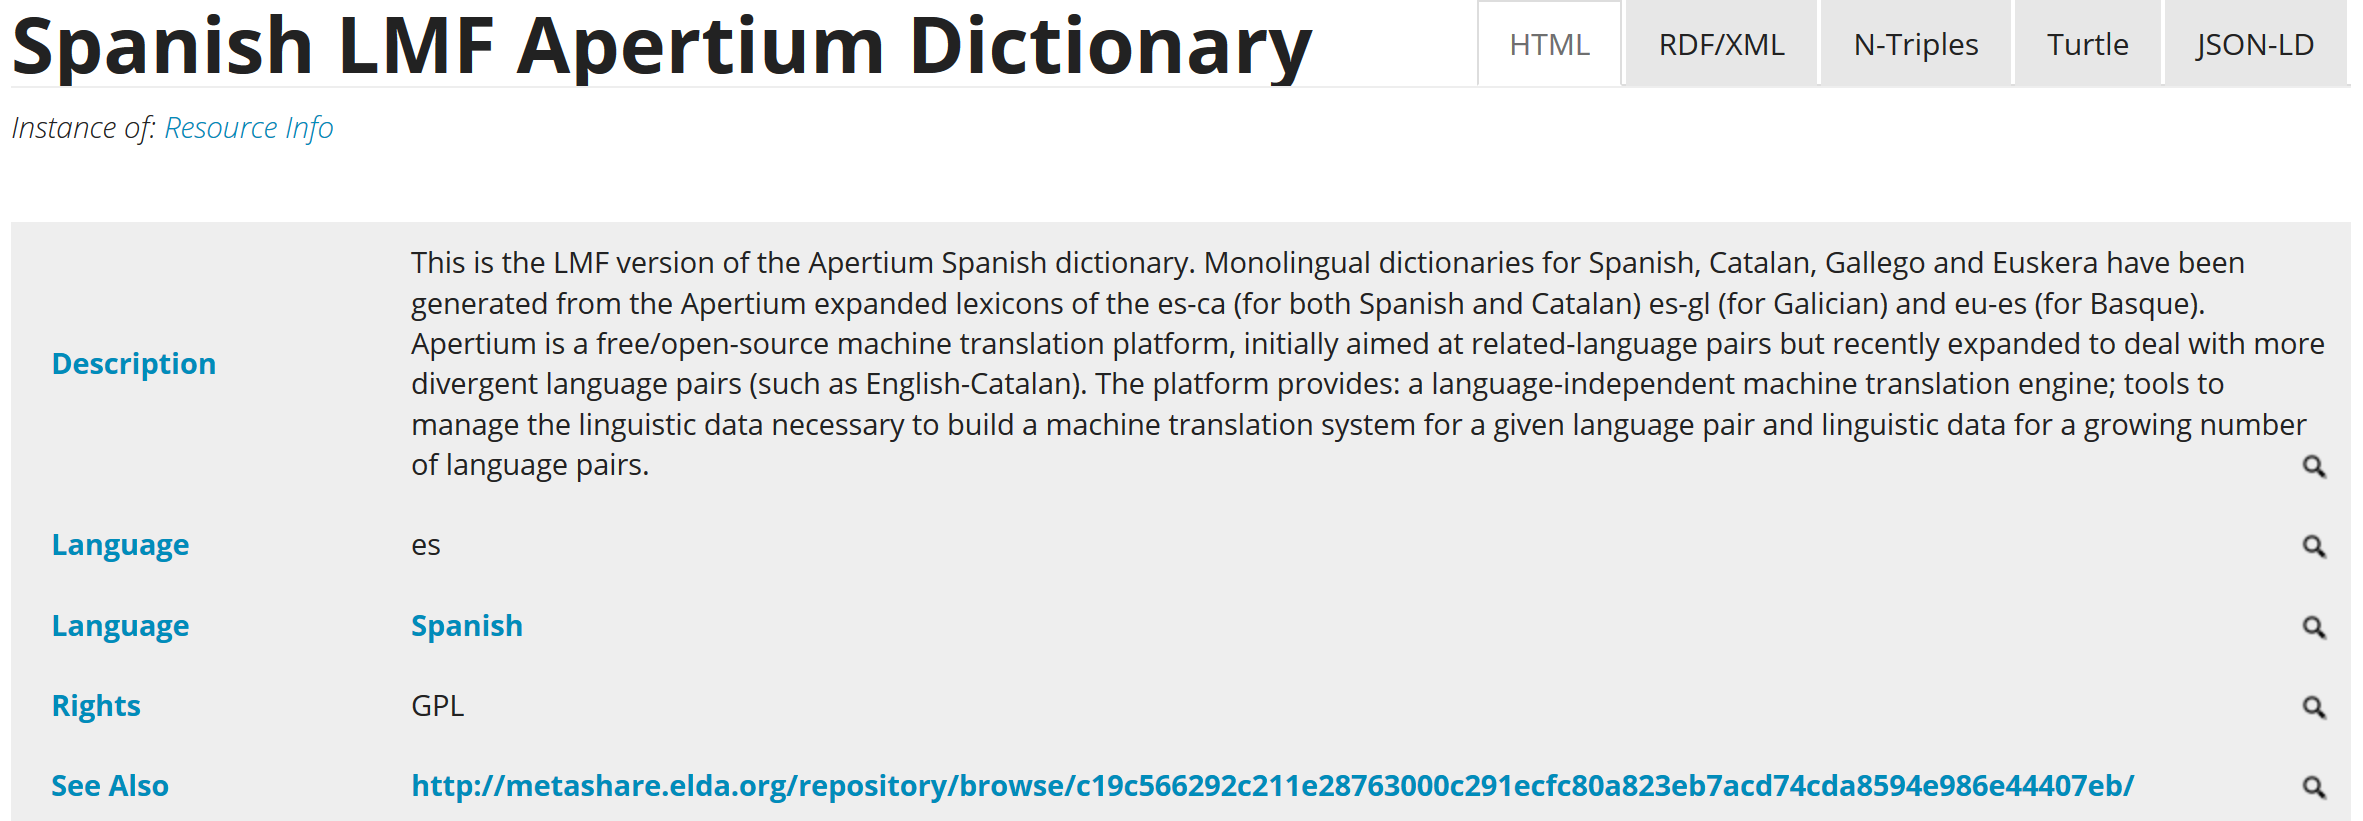
\includegraphics[width=\textwidth]{img/linghub-screenshot.png}
\caption{A screenshot of the Linghub interface\label{fig:screenshot}}
\end{figure*}

Proper access to the dataset requires a pleasant and functional interface and
the design of such an interface should not be ignored. As such, we provide
Linghub as a website that allows both humans to see the data in the form of HTML
pages and for computers to access that data in the following formats: RDF/XML,
Turtle, N-Triple and JSON-LD. Simple templates are used that render the data in
HTML so that human users can obtains a consistent view of the data, from all of
the sources displayed in Linghub. Furthermore, we provided some extra
mechanisms, by which users could access the data

\begin{description}
    \item[Faceted browsing] Users can choose to slice datasets up by a number of
        elements including language, rights, type, creator, source, contributor
        and subject. The users can see all relevant dataset as well as querying
        specific parameters
    \item[Free-text search] The most common search method employed on the Web is
        free-text search and we employ this by building a search interface that 
        indexes all the literal values in the data and allows free search over
        them. In addition, for certain values, especially languages we added in
        the values of the literals and indexed them\todo{note sure this is
        working}.
    \item[SPARQL search] Finally, we enabled SPARQL search for advanced and
        automated users, that as we show in the evaluation improves the ability
        of clients to find relevant results. For performance reasons, we limit
        the expressiveness of queries to those that are likely to be easy to
        compute. The endpoint by default returns results in
        JSON~\cite{seaborne2013sparql}.
\end{description}

\section{Evaluation}
\label{evaluation}

\subsection{Evaluation Methodology}

To evaluate the usefulness of Linghub based on actual needs for linguistic 
resources, all questions for language resources posed on the Corpora Mailing 
List (CML)~\footnote{\url{http://mailman.uib.no/public/corpora/}} since January
1st 2015 have been examined. After ruling out a small subset of questions on the
mailing list that were too underspecified and unclear to be operationalised even
for a completely manual search, a catalogue of 23 request was assembled. Each
request poses a number of constraints on the data being searched. Constraints
typically contain the \emph{type} of the resource like corpus, lexicon, tool or
service; the language the resource is applicable for; the relative size of the
resource measured in various metrics like word count and additional qualities,
like intended use.  

Each request was then searched for in Linghub using both, the standard search
\footnote{To make the search for suitable interface queries more time-efficient,
    a prototype for the query was first developed testing equivalent SQL queries
    against the SQLite database schema backing the YuZu TripleBackend, since for
    example the user interface itself offers no straightforward way to find out
    about the total number of matches for a query without traversing the
pagination}
interface as well as SPARQL queries. This covers both relevant audiences:
Standard users like most linguists and developers looking for data without being
familiar with SPARQL, and Semantic Web experts fluent in SPARQL. Results of the
queries were counted and each was evaluated as relevant, irrelevant or related
\footnote{``related'' meaning that some constraints were not or not fully met.}
to the query. The original request \#6 was skipped, because the evaluators could
not agree what exactly constitutes a ``corpus suitable for training hierarchical
classification models''. 

\subsubsection{Limitations}

The methodology chosen can only evaluate Linghub in a limited way. The first and
most important limitation is the biased sample of queries. People asking for
help on the Corpora Mailing List will most probably already have searched using
standard means, such as Google or repositories known to them. This can limit the
queries to very specific requests, that are complicated to find answers for. The
technical expertise of the users and, consequently, their more specific
requirements also contribute to the requests being more complicated. Thus, all
but a few queries examined are expert level queries, limiting the general
applicability of this evaluation. 
Although the timespan examined constitutes a reasonable sample with six months
of mailing list requests analysed, the number of queries is quite low. However,
as section 2 will detail, their overall type and language profile matches
available Linghub data.
Due to the complicated nature of the requests, translating them from natural
language to concise and reasonably narrow queries to the search interface
respectively SPARQL constitutes another hurdle, that is hard to control for. 
Search was furthermore conducted by two persons, whose interpretation of the
meaning of the query and thus the relevance of the resources found may vary. 

\subsection{Resource request analysis}

The requests were analysed in regard to the constraints they express. All
queries expressed at least 2 constraints, usually regarding the resource type
and the preferred language of the resource. Requested resource types were
limited to corpora, tools, lexical and spoken resources. Corpora were requested
in nearly 70\% of the cases, followed by tools (17.4\%) and lexical resources
(13.0\%). As seen in Figure 1, this resembles the resource distribution in
Linghub, where 71.5\% are corpora as well. 
Most language restrictions asked for one language or made no specification at
all. The falling number of requests for higher language restriction count with a
small rise above 20 languages again resembles the resource distribution in
Linghub, that also shows a power law distribution of resource language count.
The rise above 20 languages can be explained by the use of European corpora that
contain all European languages.  

\todo{Markus: Can you provide original images for this paper?}

\begin{figure}
    markus to upload
    \caption{\label{fig:req-by-type}Linghub resources and resource requests by
type}
\end{figure}

\begin{table}
    \begin{tabular}{c|c}
    Language count constraint & Number of requests \\
    \hline
    1                         & 8                  \\
    2                         & 1                  \\
    3                         & 2                  \\
    4                         & 1                  \\
    \textgreater 20                      & 2                  \\
    unspecified               & 7                  \\
\end{tabular}
    \caption{\label{tab:language-constraints}  Language constraints in requests
        and resources available in Linghub covering specific numbers of
    languages}
\end{table}

\begin{figure}
    markus to upload
    \caption{\label{fig:language-constraints} Language constraints in requests
        and resources available in Linghub covering specific numbers of
    languages}
\end{figure}

Besides these common constraints, most requests also define at least one further
restriction. For corpus requests, a common restriction is having a large size in
number of words. Specifically, “gigaword” corpora or corpora with “billions of
words” are highly searched for. Surprisingly, only one request explicitly
limited the license to free and open resources. Further restrictions mention the
type of annotation (for example manually checked or annotating specific
features), the feature set of a tool or service or the semantic content of the
resource. These restrictions can only be judged by first doing a full-text
search in the description of the resources, then reading these descriptions and
judging their appropriateness. Thus, the assessment of relevance or relatedness
of resources found during search is subjective and may not always be comparable.


\subsection{Standard search interface}

While trying to express the facets of the questions from the CML in Linghub,
several shortcomings both of the browsing functionality and the `simple' search
became apparent. 
The inability to declare combined restrictions for several facets (description,
language, rights, \ldots) simultaneously is presumably the most crucial limitation
for both the browsing interface and the search form. Online catalogues usually
either offer alternative search form for `advanced' users where a flexible
number of pairs of field specifiers and a corresponding search patterns can be
defined, whose constraints will be combined by boolean operators or complex
search patterns can be defined, allowing for sub-patterns that are matched
against solely against specified record fields, e.g.:

\begin{verbatim}
(title:corpus OR description:corpus) AND 
  (description:(“part of speech” OR pos)) AND 
  (language:(deu* OR german))
\end{verbatim}

Since the overwhelming majority resource requests from the CML involved ‘soft’
constraints that can only be expressed with full-text patterns against resource
descriptions, additional structured information about language or rights could
not be harnessed during the query (as the sole facet choice already had to be
used for the description). Especially for formulating multiple ‘soft’
constraints against the resource descriptions the full text search capabilities
from SQLite exposed in the search interface proved very useful. 
%These
%possibilities should be advertised more prominently to users\footnote{
%    During the evaluation process one of the evaluators only became aware of the
%    availability of full-text query operators when examining YuZu source code to
%    obtain a better understanding of other aspects of the behaviour of the
%Linghub platform.}.  

Some of the facets offered by Linghub are naturally textual (e.g., title,
description, creator), but others are rather categorial with a limited set of
options (e.g., resource type, language). The usability of the search interface
could benefit if constraint formulation for the categorial facets would be
designed in a manner different from a simple full-text search field, presenting
the set of options and allowing selection of the desired subset of suitable
values for the resource request to be formulated. Such facilities are already
implemented in the browsing interface, but only a sole option can be selected
there at the moment.

Currently also categorial facets are to be queried with the full-text
facilities, which on the one hand allows for selecting combination of allowed
categorial values, but requires knowledge of appropriate matching string values.
One extreme example of this limitation is the usage of the language facet for
the current implementation: the full-text pattern is matched against the
lexvo-URI representations of the ISO 639-3 language codes. So the search
``language=german'' will yield (perhaps surprisingly) no results. The desired
restriction has to be framed as language=deu, which might be perceived as
unintuitive for uninformed first-time users. 

Currently the search form does not ensure that text pattern are matched
exclusively against title and description values for resources with matching
languages this can be problematic due to homographs and cognates shared by
English, Spanish, French etc.  

Excluding the queries that did not yield results, on average 10.8\% of the
results were relevant, 11.9\% were related and 77.3\% were irrelevant. The high
share of irrelevant search results does not come surprising, as the queries
formulated for evaluation generally were rather open than restrictive in many
cases to favour recall over precision, as one can assume that potential users of
language resources will be willing to invest a bit more time to manually sift
through an acceptable amount of additional false positives rather than risk
missing information of an additional potentially useful resource. 

\begin{figure}
    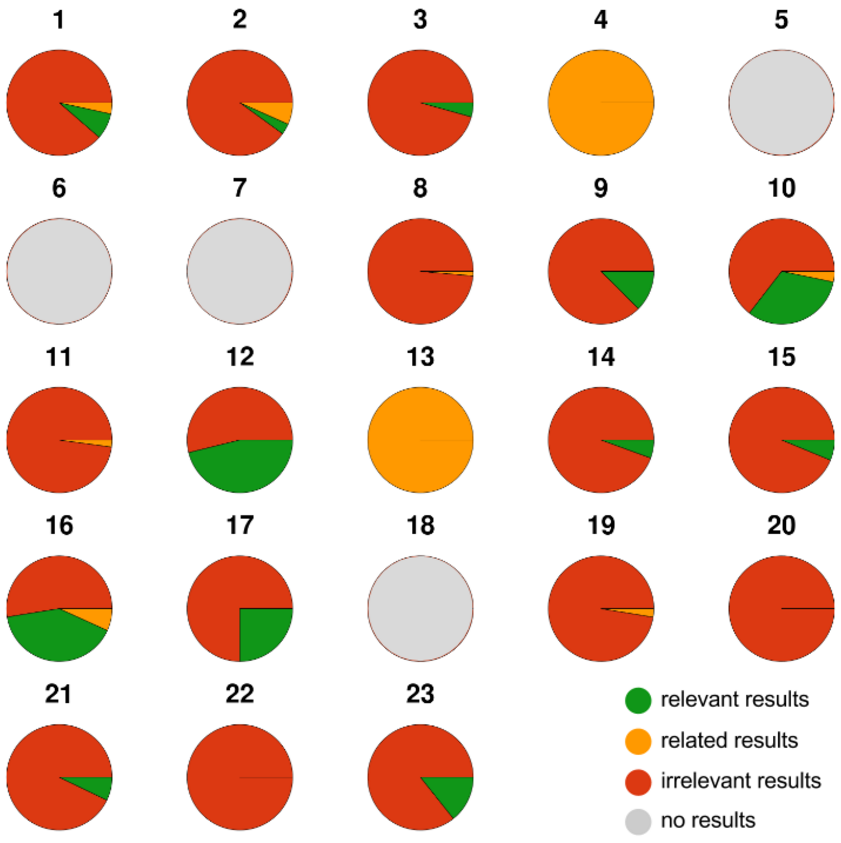
\includegraphics[width=\textwidth]{img/eval_rel_interface.png}
    \caption{\label{fig:freetext-rel} Percentages of relevant standard interface
    search results}
\end{figure}

\subsection{SPARQL search}

While the standard search interface presents the default access point to the
Linghub knowledge base, SPARQL search is regarded as ``advanced search''. Using
SPARQL naturally solves most issues of the standard search interface, as it can
be used for granular search in arbitrary literal fields and natively provides
logical operators for filters to combine them. If values are modelled as
classes, the user does not have to use string matching but can use object
relations, working on a well-defined, semantic level. The only disadvantage of
SPARQL is its inaccessibility to most linguists that don’t have firm knowledge
in database query languages.  

SPARQL queries were written and executed using the downloaded Linghub dump for
convenience. The queries and detailed results can be found in the appendix.

Figure 4 shows the results for each of the queries. Excluding queries 6 and 18
that yielded no results, on average 21.5\% of the results were relevant, 10.7\%
were related and 67.8\% were irrelevant. Roughly a quarter of the queries
failed, yielding no relevant results or no results at all. In general, this can
be considered as a good result, taking into account the complicated nature of
the queries. Specifically, it indicates that the more granulated means SPARQL
provides to the user lead to more accurate results. 

\begin{figure}
    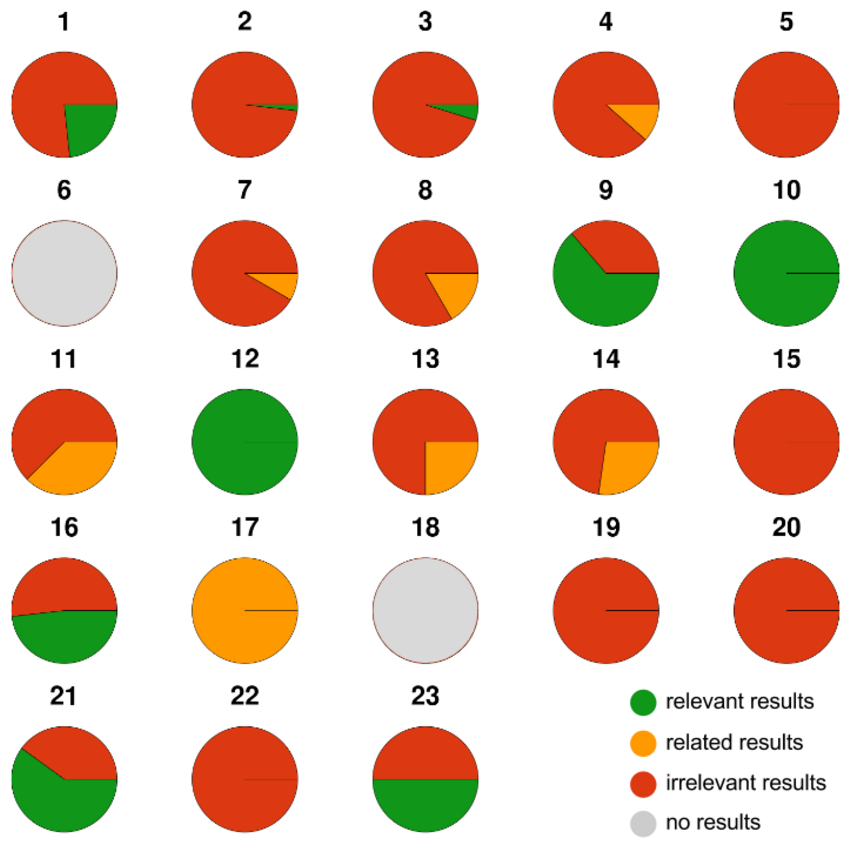
\includegraphics[width=\textwidth]{img/eval_rel_sparql.png}
    \caption{\label{fig:sparql-rel}Percentages of relevant SPARQL search results}
\end{figure}

Language proved to be the most restricting constraint, leading to most irrelvant
results, even if other constraints are met. Although SPARQL was used to
granularly restrict the 
languages by leveraging the \texttt{dc:language}, queries were not limited to
this relation but also incorporated searching for the language name in the
\texttt{dcterms:description} to increase recall. 
Size was another important constraint that was never fully met. If size was a
restriction, it always was in the range of billions of words, excluding all
relevant corpora as too small. Corpora with millions of words were counted as
related. It would be helpful to express this measure as an own datum\todo{I
don't understand this - JPM} in Linghub
to help future searchers. However, it could only be automatically acquired by
retrieving and parsing the resources, taking into account their format. This
approach would thus be limited to open resources with detailed metadata. Again,
description texts were used to retrieve hints on corpus size.
One large advantage of SPARQL was being able to explicitly address fields such
as distribution and license information, allowing to filter for free and open
resources, as well as links to the data itself. The selection of the queries in
CML reduced this use-case to one case, but it seems to be an important and often
overlooked facet of data acquisition. 

\subsection{Data Completeness and Quality}

To obtain statistics on data completeness, relative frequencies of Linghub
resources carrying at least on property-value pair for the various facets
offered by the search frontend were determined. The basic quantity of Linghub
resources was defined as all URIs in the Linghub dataset with the
linghub.lider-project.eu hostname appearing in subject position of at least one
triple. Figure \ref{fig:reqinfo} presents the aforementioned relative frequencies:



% we stash the image here to get it's height for properly aligned minipages  
\newsavebox{\imgbox}
\savebox{\imgbox}{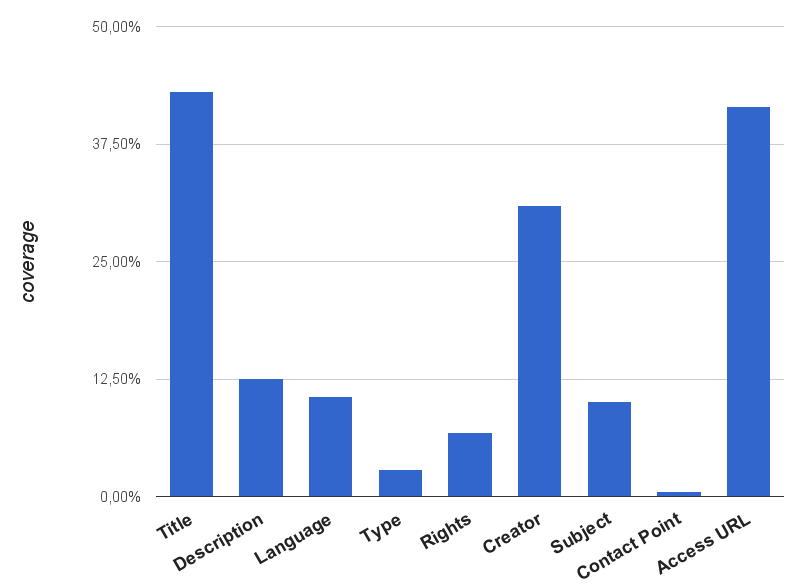
\includegraphics[width=0.53\textwidth]{img/eval_facet_coverage.png}}
\showthe\ht\imgbox 
\begin{figure}
    \begin{minipage}[l][\ht\imgbox][t]{0.45\textwidth}
    \begin{tabular}{lrr}
      required facet & abs. freq & rel. freq. \\
      \hline
      (none)         & 444606    &  100\%     \\
      Title          & 191355    & 43.04\%    \\
      Description    & 55697     & 12.53\%    \\
      Language       & 47357     & 10.65\%    \\
      Type           & 12780     &  2.87\%    \\
      Rights         & 30165     &  6.78\%    \\
      Creator        & 137675    & 30.97\%    \\
      Subject        & 44725     & 10.06\%    \\
      Contact Point  & 2436      &  0.55\%    \\
      Access URL     & 184452    & 41.49\%    \\
    \end{tabular}
  \end{minipage}
  \begin{minipage}[r][\ht\imgbox][t]{0.55\textwidth}
      \usebox{\imgbox}
  \end{minipage}
  \caption{\label{tab:reqinfo} Portions of Linghub resources  carrying at
      least one property value for the respective required facet}
  \label{fig:reqinfo}
\end{figure}
 
These statistics reveal significant variation in coverage over the various
facets, that can result in unexpected recall when relying on facets with low
coverage. To illustrate this with an example: 444 Linghub resources containing
keywords `spanish' or `spain' in their description also carry a corresponding
dc:language property. On the other hand 493 resources with aforementioned
keywords in the description do not carry a dc:language attribute. Although the
mere appearance of the keywords are not conclusively indicative that the
resource should be counted to the corresponding language, the majority of the
latter resources appeared to be Spanisch or relevant for Spanish when examining
a 10\% sample. Albeit these resources are currently ruled out implicitly when a
user uses the filter option for language. Combined usage of the language
property values when present and fall-back to text-matching on title and
description, as used in the SPARQL queries, can mitigate this problem. Using the
free text pattern syntax with field specifiers, this procedure can be sketched
as: 

\begin{verbatim}
language:spa OR title:(spanish OR spain*) OR 
  description:(spanish OR spain*)
\end{verbatim}

Analogous text-pattern fallback strategies might be employed for other
properties with low-coverage (e.g. type) and could be offered as on-demand
option in the search interfaces. 

Several of the examined resource requests from the CML asking for corpora also
formulated minimal requirements for their size. About 4000 resources listed in
Linghub carry property-value pairs for numeric values quantifying their size
according to a specified unit. Excluding also cases where the unit is not
clearly specified or where the size value is just a sentinel value for ‘no
available’, about 2490 resources with well defined, structured size information
remain (all of these originate from META-SHARE).  Increasing this coverage
towards a substantial portion of corpus resources indexed in Linghub would be
quite beneficial. However, although missing size information could probably be
extracted from description texts for many resources, achieving a satisfactory
level of correctness of such a process would presumably require a prohibitively
great extend of manual annotation and curation


\section{Conclusion}
\label{conclusion}

\todo{JPM to finish}

%\bibliographystyle{spbasic}      % basic style, author-year citations
\bibliographystyle{spmpsci}      % mathematics and physical sciences
%\bibliographystyle{spphys}       % APS-like style for physics
\bibliography{linghub-jlre}   % name your BibTeX data base

\end{document}
